% coming soon

We have implemented our switching continual approach in the MAPSIM
environment~\cite{brenner:nebel:jaamas09}. Our implementation is able
to use several underlying planning systems. We have also extended
MAPSIM system so that it can parse DTPDDL, and perform successive
estimation of the underlying belief-state using
\system{dlib-ml}~\cite{king:2009} for inference.  In this evaluation
we use our own version of Fast Downward~\cite{fast-downward} for
sequential sessions. We have extended that system to support actions
with success probabilities. In our evaluation Fast Downward is run
with the cyclic causal graph heuristic using an A* search or weighted
A* (with weight 5). We use A* for easy problems and WA* for more
difficult problems where A* is ineffective. Contingent sessions use
our own forward search procedure.


\Omit{ We then perform multiple tests with different limits for the
  belief-space size in contingent sessions.  Higher limits should
  cause longer planning times but be beneficial to plan quality as
  more contingencies can be taken in to account by the POMDP planner.
}

In order to evaluate our system, we have also implemented a baseline
approach in MAPSIM. Rather than invoking a contingent session when a
switching action $\switchAction$ is scheduled for execution, the
baseline simply executes one action that can trigger a sensing outcome
determined by the precondition of $\switchAction$, and replans in the
resulting belief-state.




%% executes switching actions and replans in the
%% resulting belief state.

%% but instead of
%% creating an observation problem for the decision theoretic planner it
%% will just execute one sensing action -- assuming that this action will
%% confirm its assumption.

To test our approach we use a robot exploration domain based on a
scenario from our physical robotic system. Here, a robot is exploring
an office or living environment, and trying to report the locations of
objects to their owner. Basic types are {\tt rooms}, {\tt places} and
{\tt objects}. Places are topological map nodes that occur in rooms.
Objects, and also the robot, are always located at a place. The robot
can move around the rooms via connections between places given by a
{\tt connected} predicate. Each room has a, possibly unknown, {\em
  category} (e.g. kitchen, office, living room). Certain objects are
more likely to be located in rooms of a particular category.  For
example, a box of cornflakes is more likely to be located in the
kitchen than the office. The robot can look for an object at a place
by executing a {\tt look-for-object} action. Executing {\tt
  look-for-object} results in a noisy sensing outcome, sometimes
indicating a positive perception if the object is there. We have that
some objects are harder to detect than others. Finally, if the robot
is in the presence of a human, it can ask what type of room it is
currently in, however conducting a dialogue is more costly than
running a vision algorithm (cost of 8 vs costs of 3).

%%  Therefore, an instantaneous positive detection of an object is
%% not proof positive of it being there.

We perform experiments on tasks of several sizes. The objective is to
find one or more objects and report their position to the user. In
order to determine the impact of the reliability of sensing in a
comparison with the baseline, we run tests on identical problems but
changed the sensor model for the target objects: the probability for
perceiving the object if it was there went from 0.9 in the easiest
case to 0.65 and 0.4 in the average and hard cases respectively. In
addition, we test how our system performs in tasks requiring indirect
sensing. Here, we gave the planner rewards for visiting a certain type
of room (e.g. kitchen or office). We did not place any humans in those
scenarios, so the only way of determining the room category is by
looking for objects typical for that room type. As this indirect
reasoning is a tasks that cannot be performed by the continual planner
alone, we did not run the baseline system on those problems.



In our evaluation we run 50 simulations in each configuration. A run
timeouts after 30 minutes (1800 seconds). The planning and simulation
models are in exact correspondence. Not all problems have a solution,
so we also examine whether or not detection of the non-existence of a
solution is important in stochastic domains.
%% 
We perform multiple tests with different limits for the
belief-space size in contingent sessions.  Higher limits result in
longer contingent planning times and higher plan quality.


Using a satisficing, optimistic serial planner in sequential sessions
makes optimising for the expected reward difficult. Only reasoning
about single traces, it is optimistic wrt the remaining costs to a
goal and pessimistic regarding the probability of reaching it. By
setting the rewards to non-extremal values has little effect on that
system. Therefore, we do not consider expected utility in our
experiments. Instead, we report average costs of the plans and the
success rate (as a ratio between solved and solvable problems).

\begin{figure}[h!]
  % \centering
  % 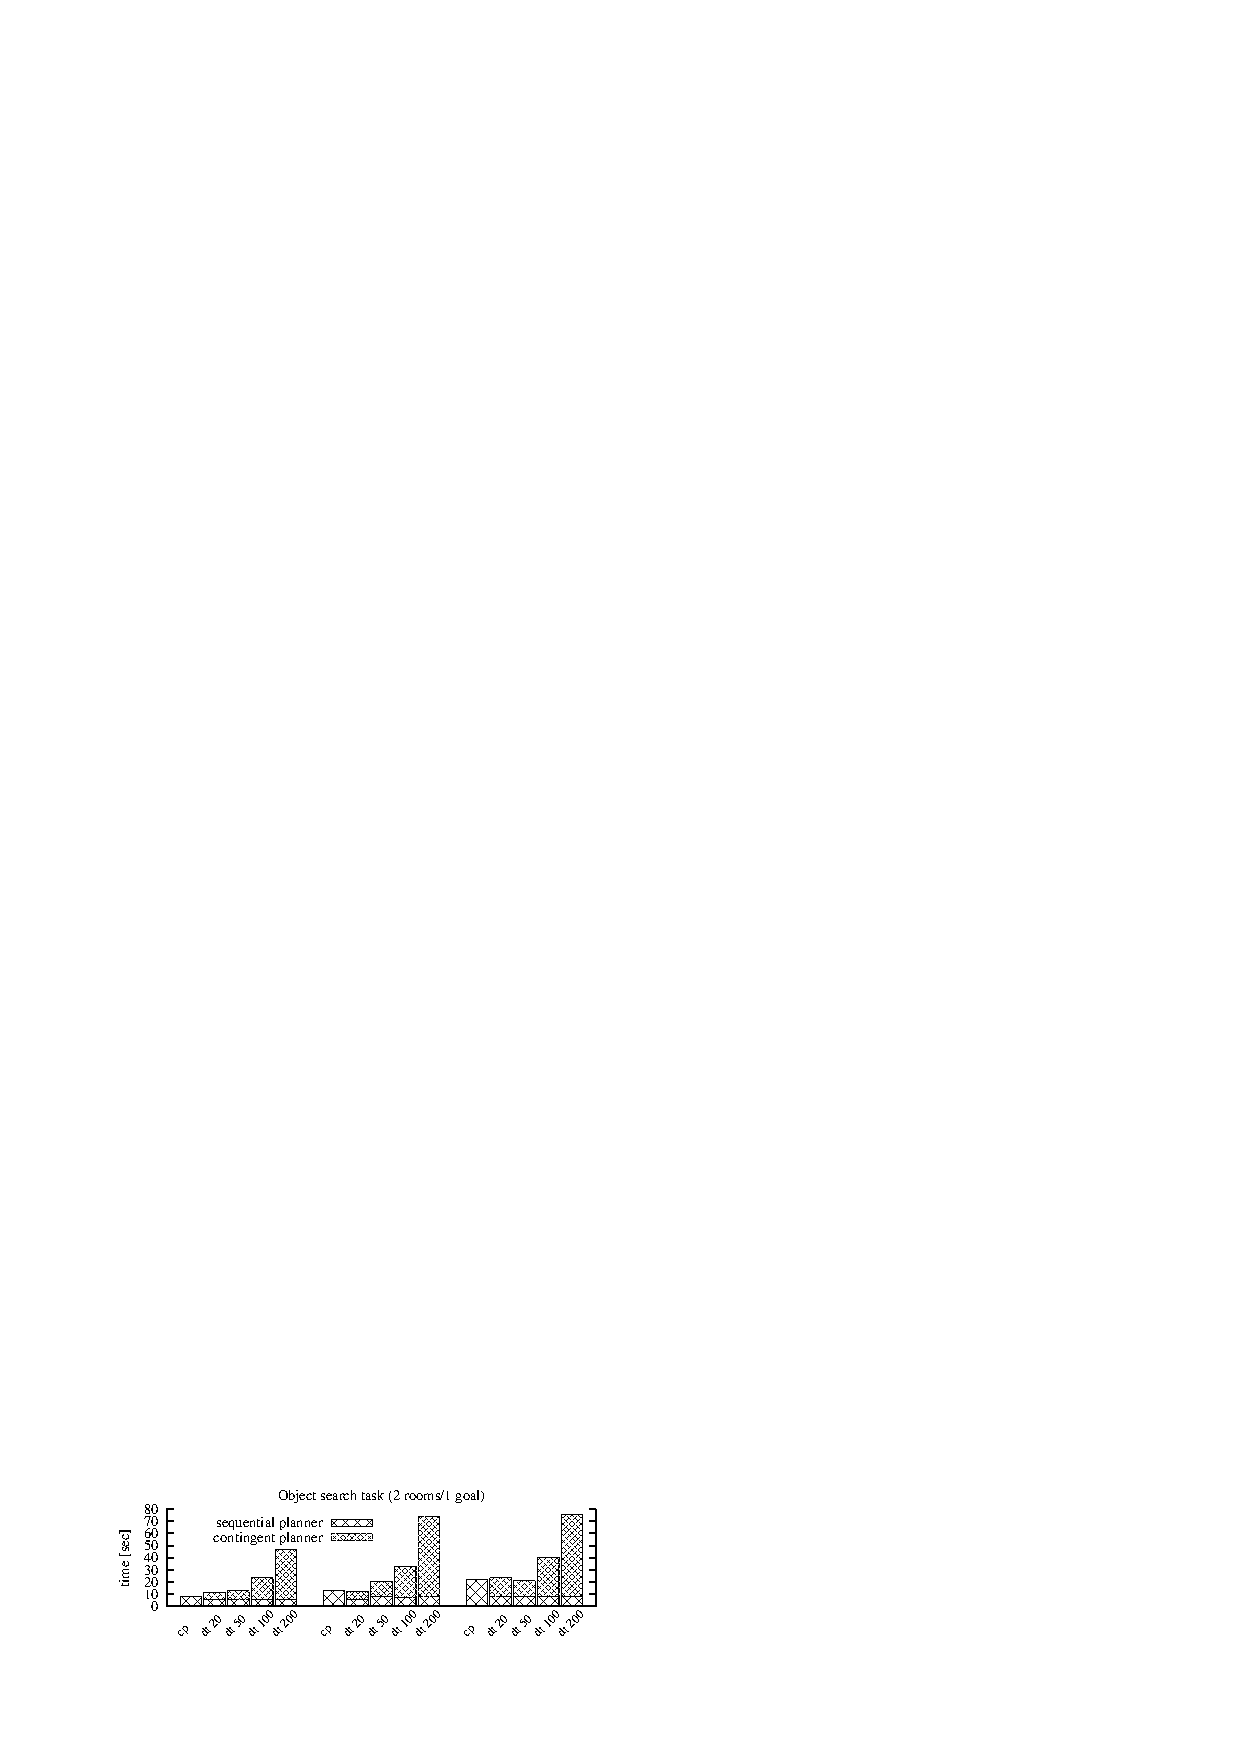
\includegraphics{dora1-time}\hfill
  % \vspace{2mm}
  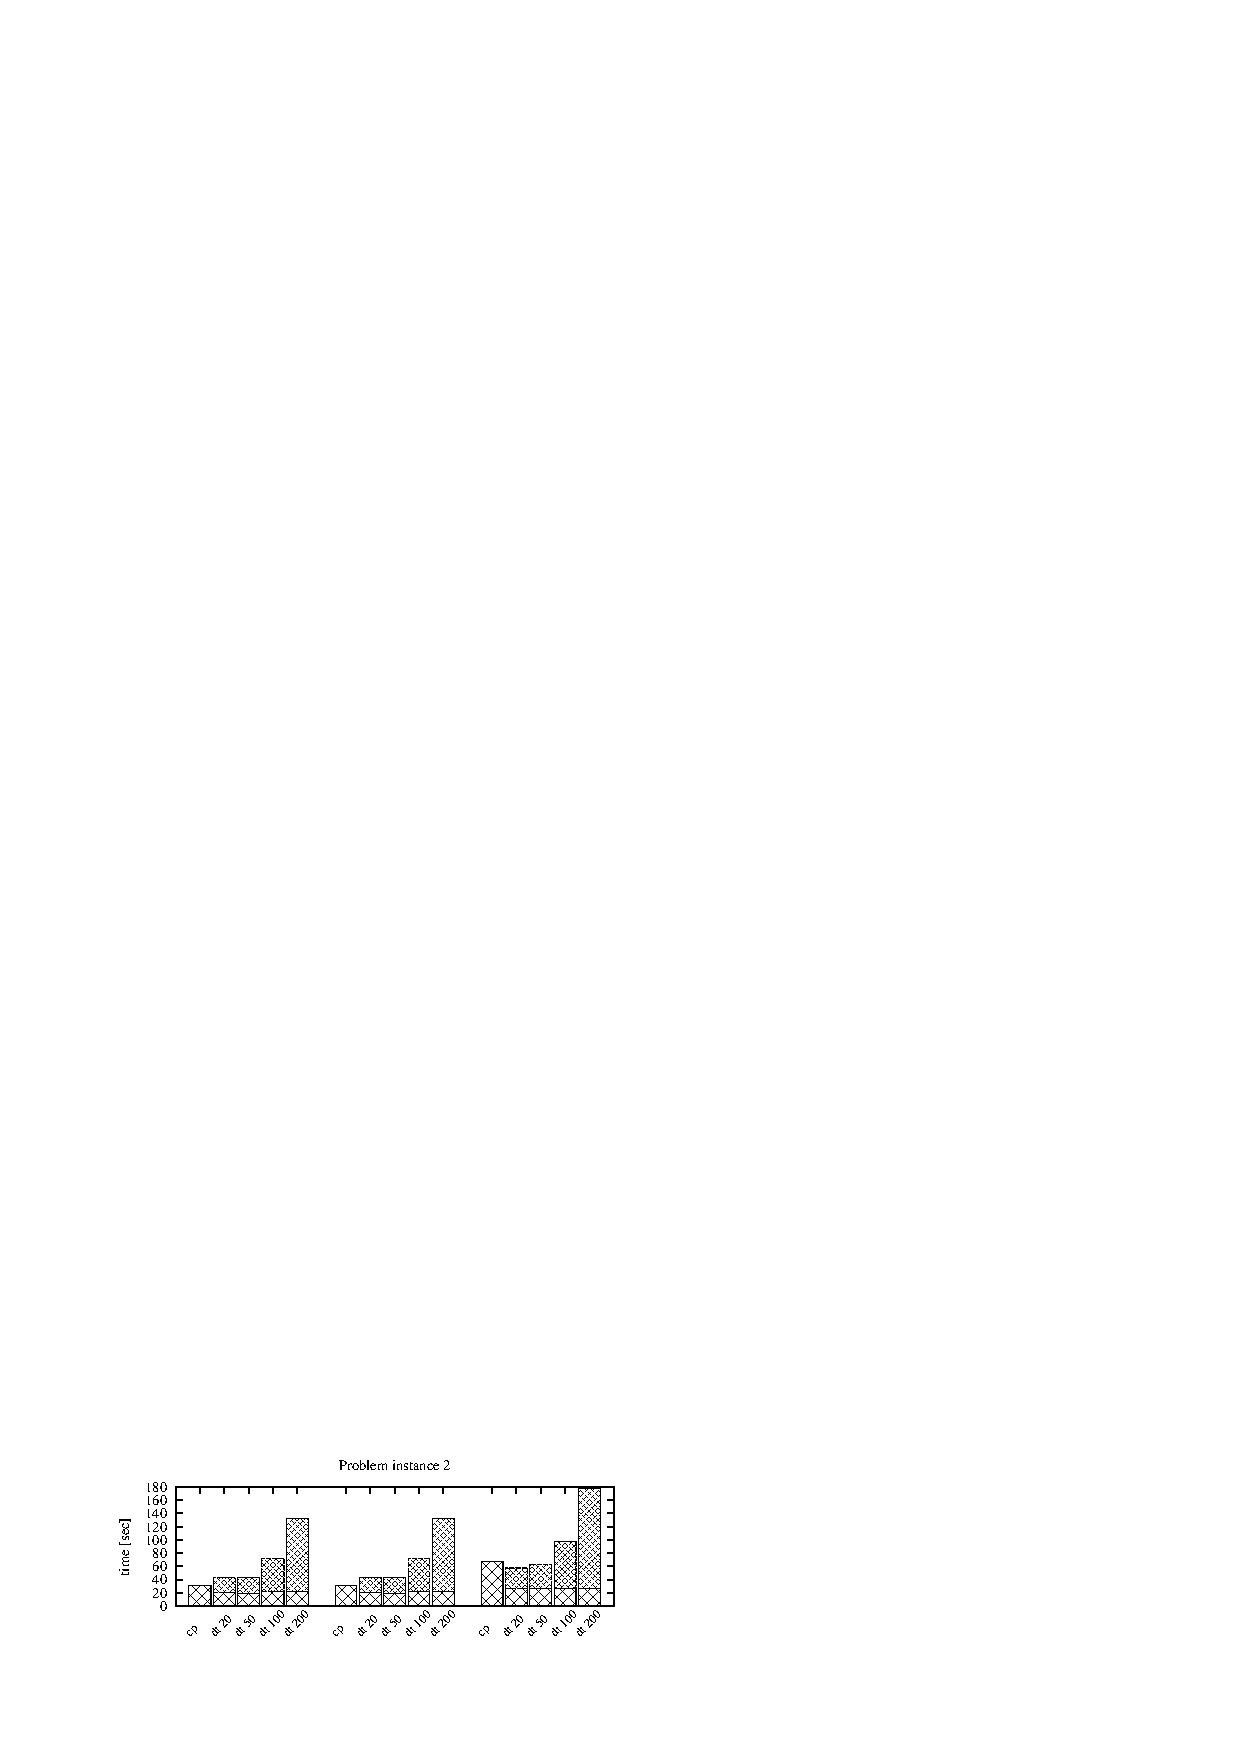
\includegraphics{dora2-time}\hfill
  % \vspace{2mm}
  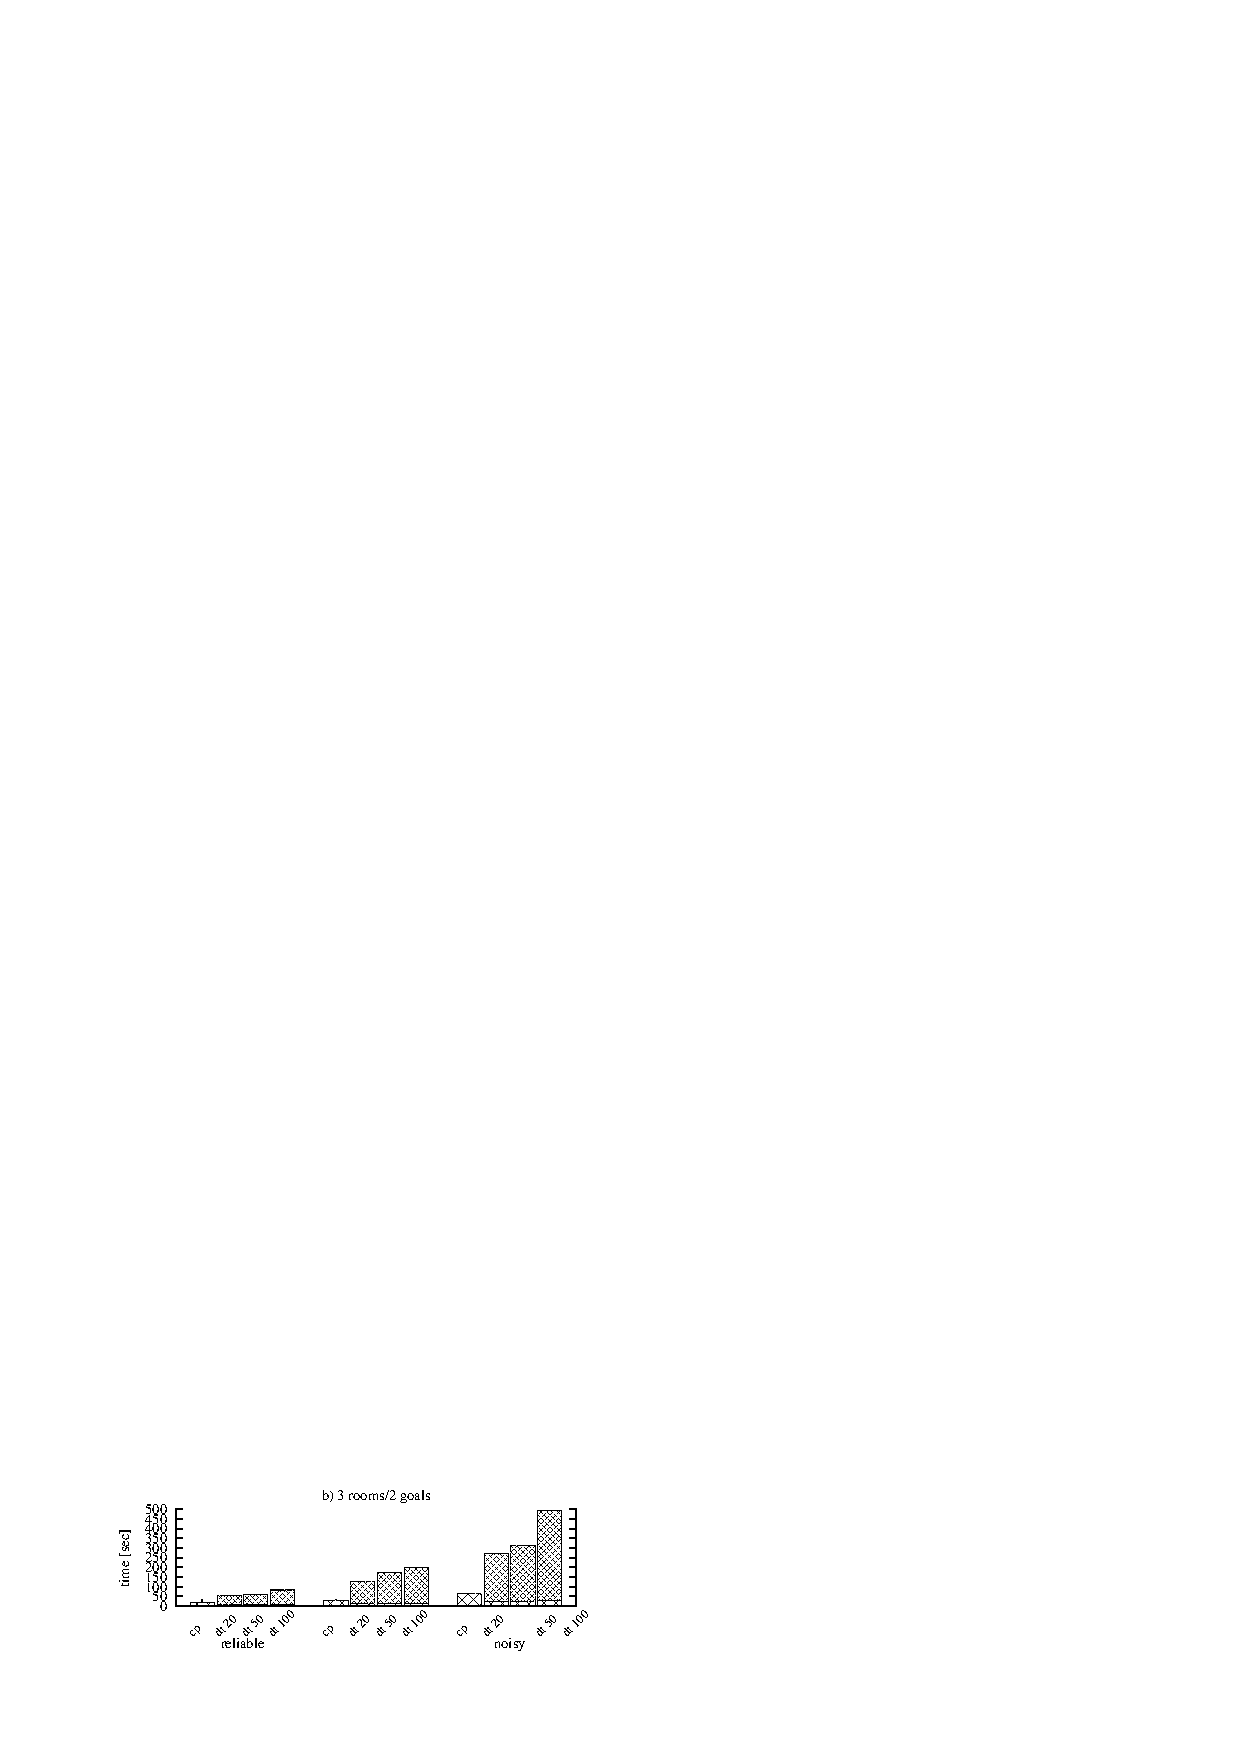
\includegraphics{dora3-time}\hfill
  % \vspace{2mm}
  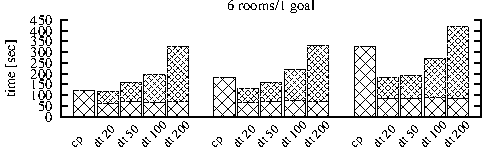
\includegraphics{dora4-time}\hfill
  \vspace{2mm}
  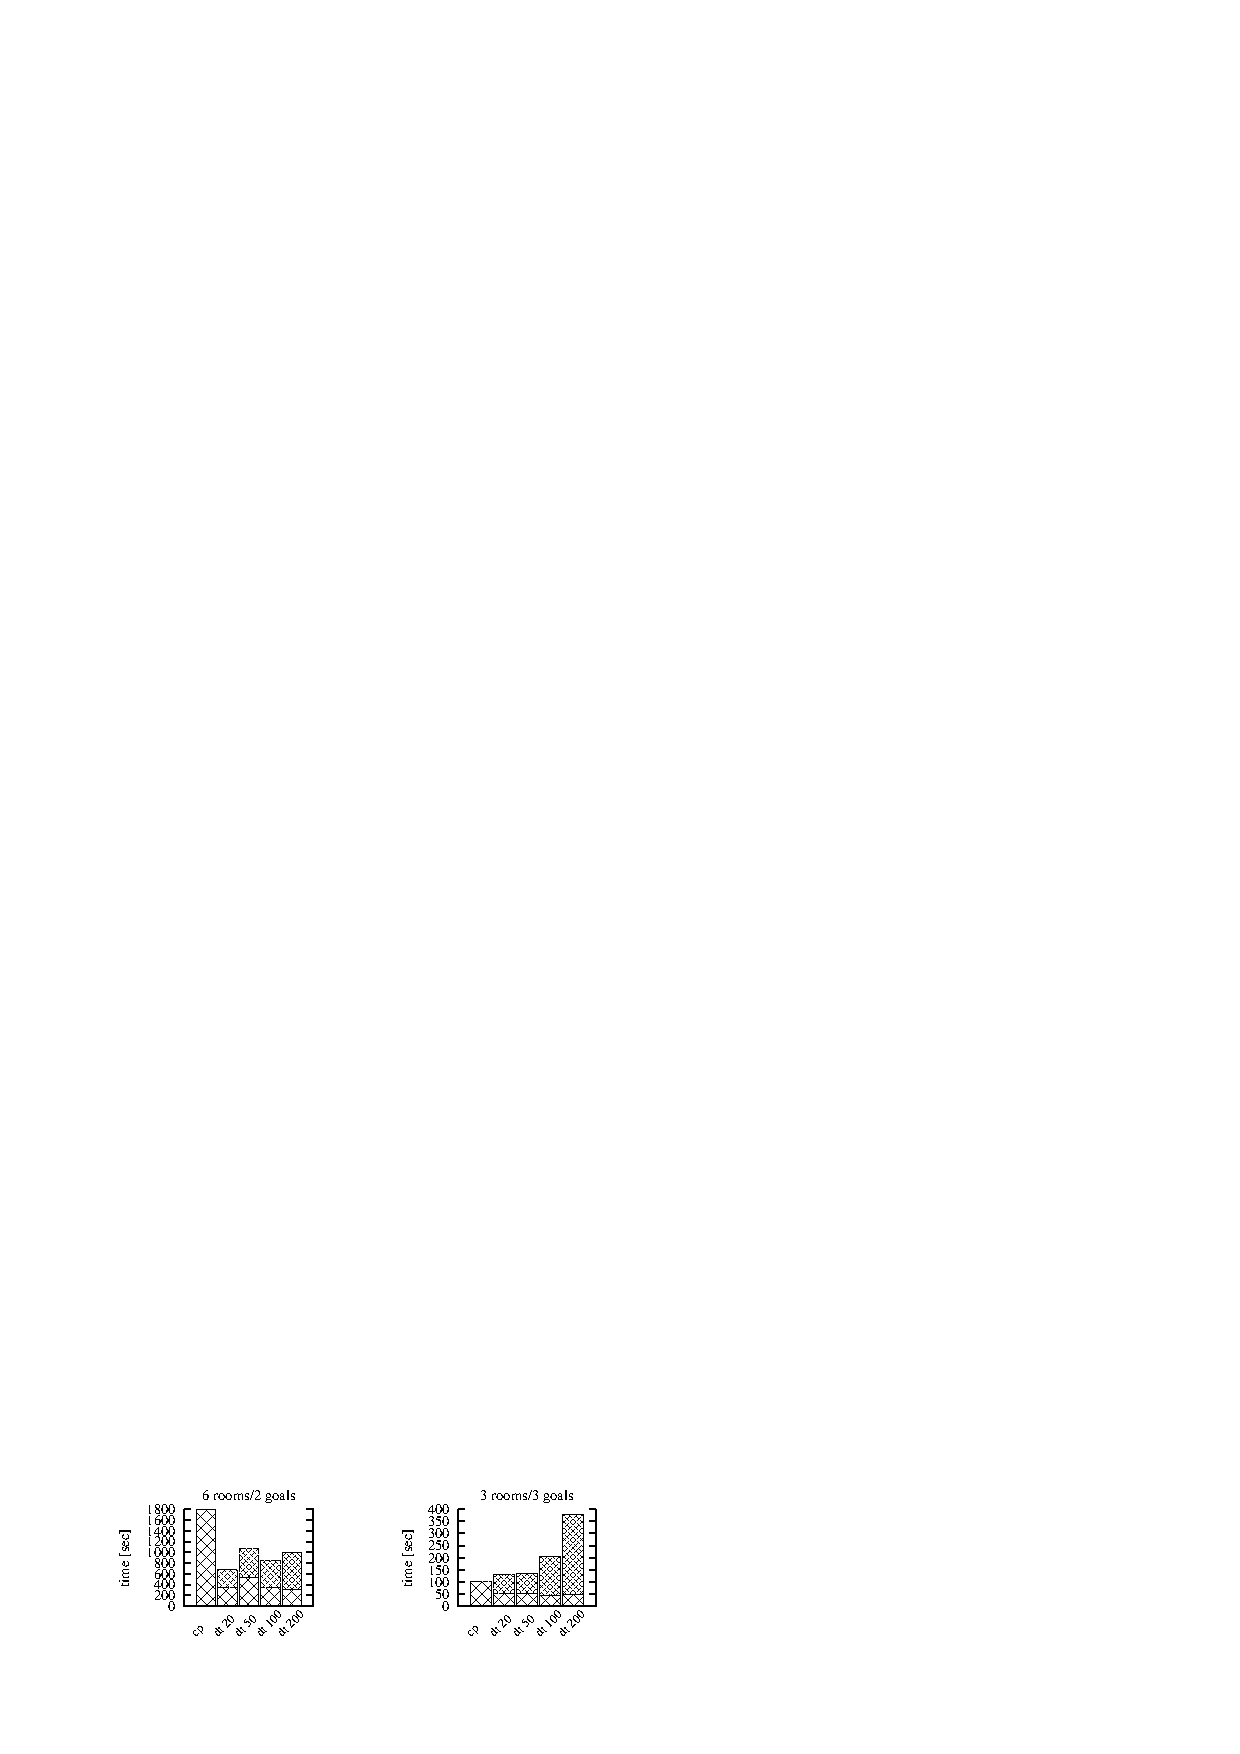
\includegraphics{dora56-time}\hfill
  \vspace{2mm}
  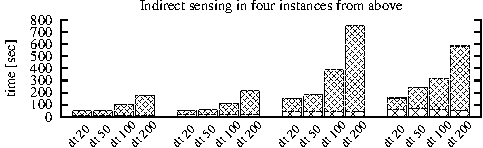
\includegraphics{dora-cat-time}\hfill
  \caption{Average runtime}
  \label{fig:results-time}
\end{figure}

\begin{figure}[h!]
  % \centering
  % 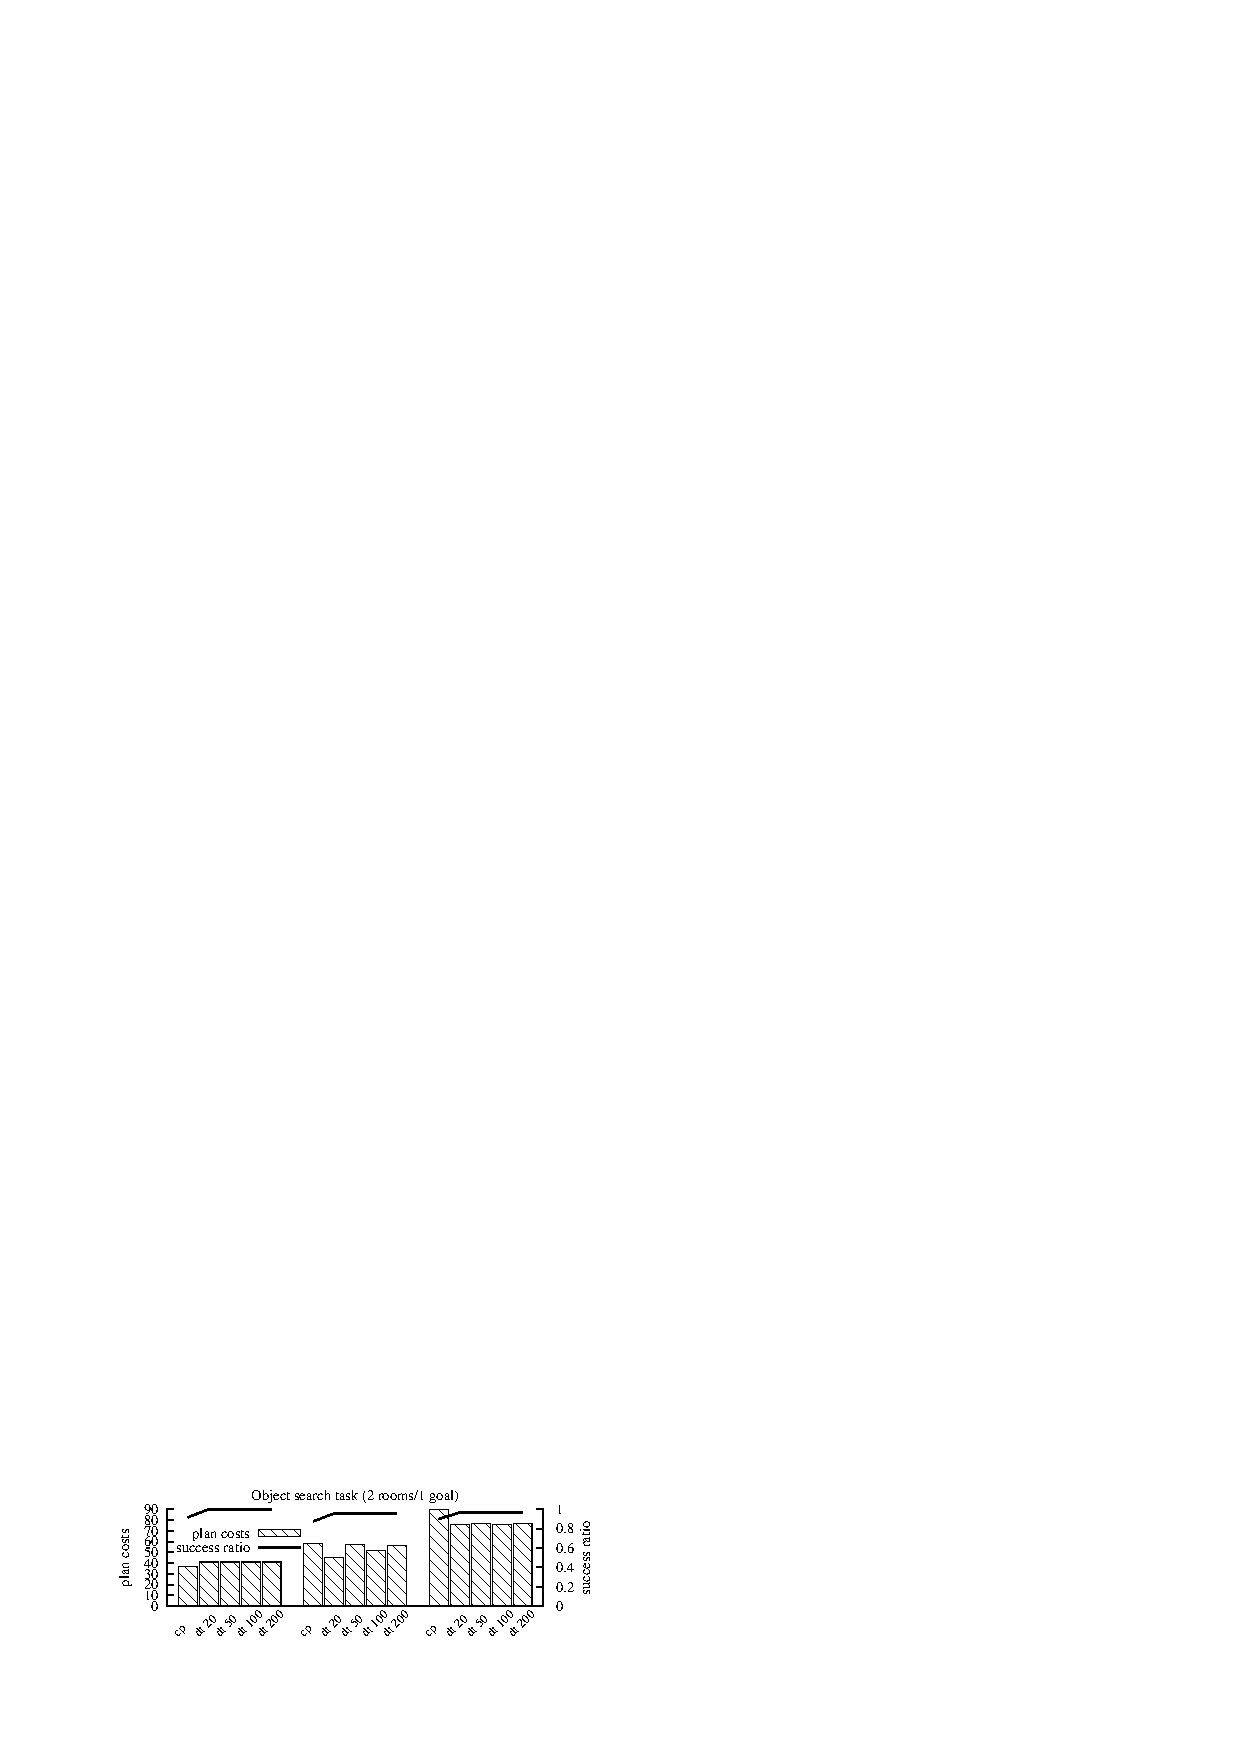
\includegraphics{dora1-quality}\hfill
  % \vspace{2mm}
  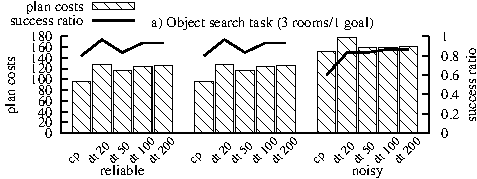
\includegraphics{dora2-quality}\hfill
  % \vspace{2mm}
  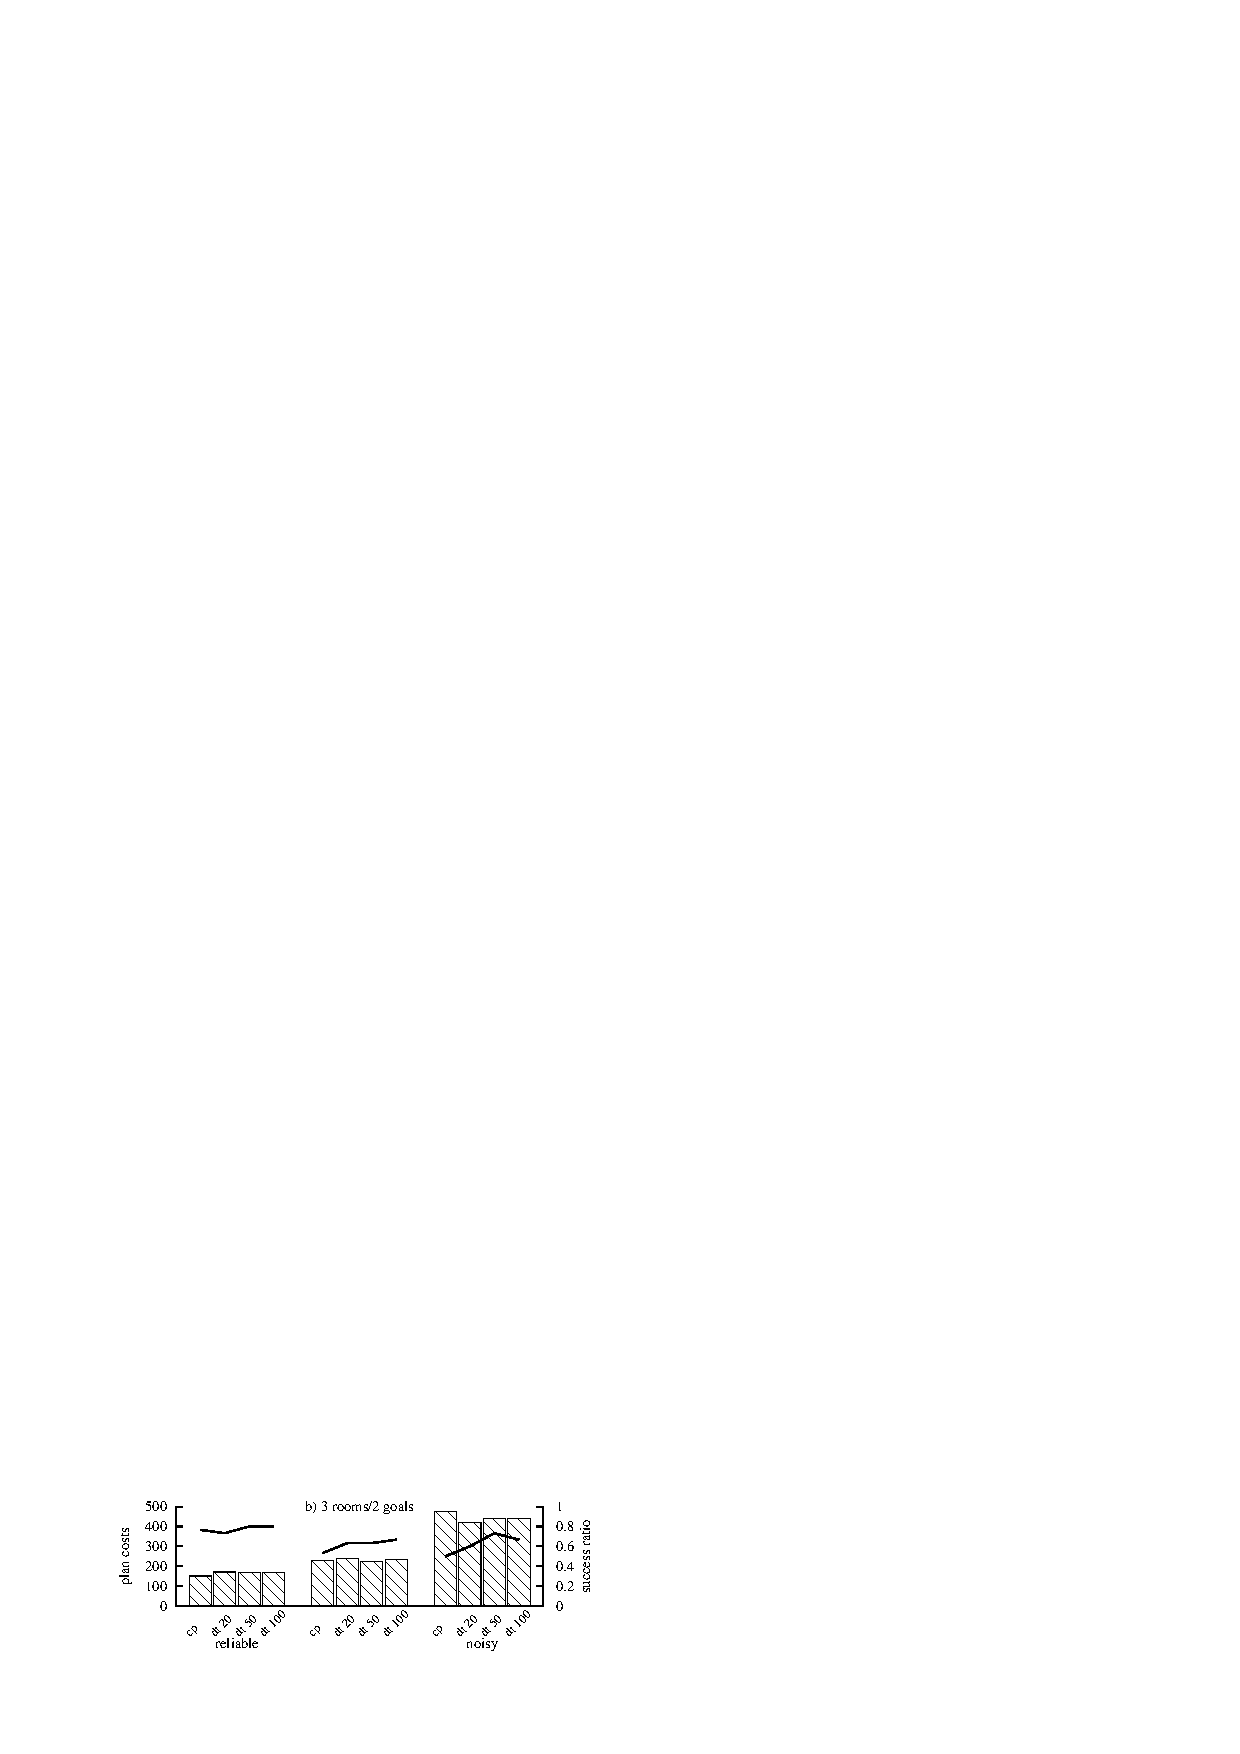
\includegraphics{dora3-quality}\hfill
  % \vspace{2mm}
  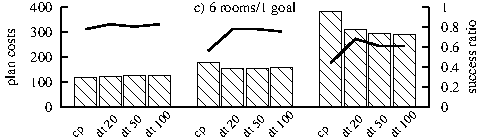
\includegraphics{dora4-quality}\hfill
  \vspace{2mm}
  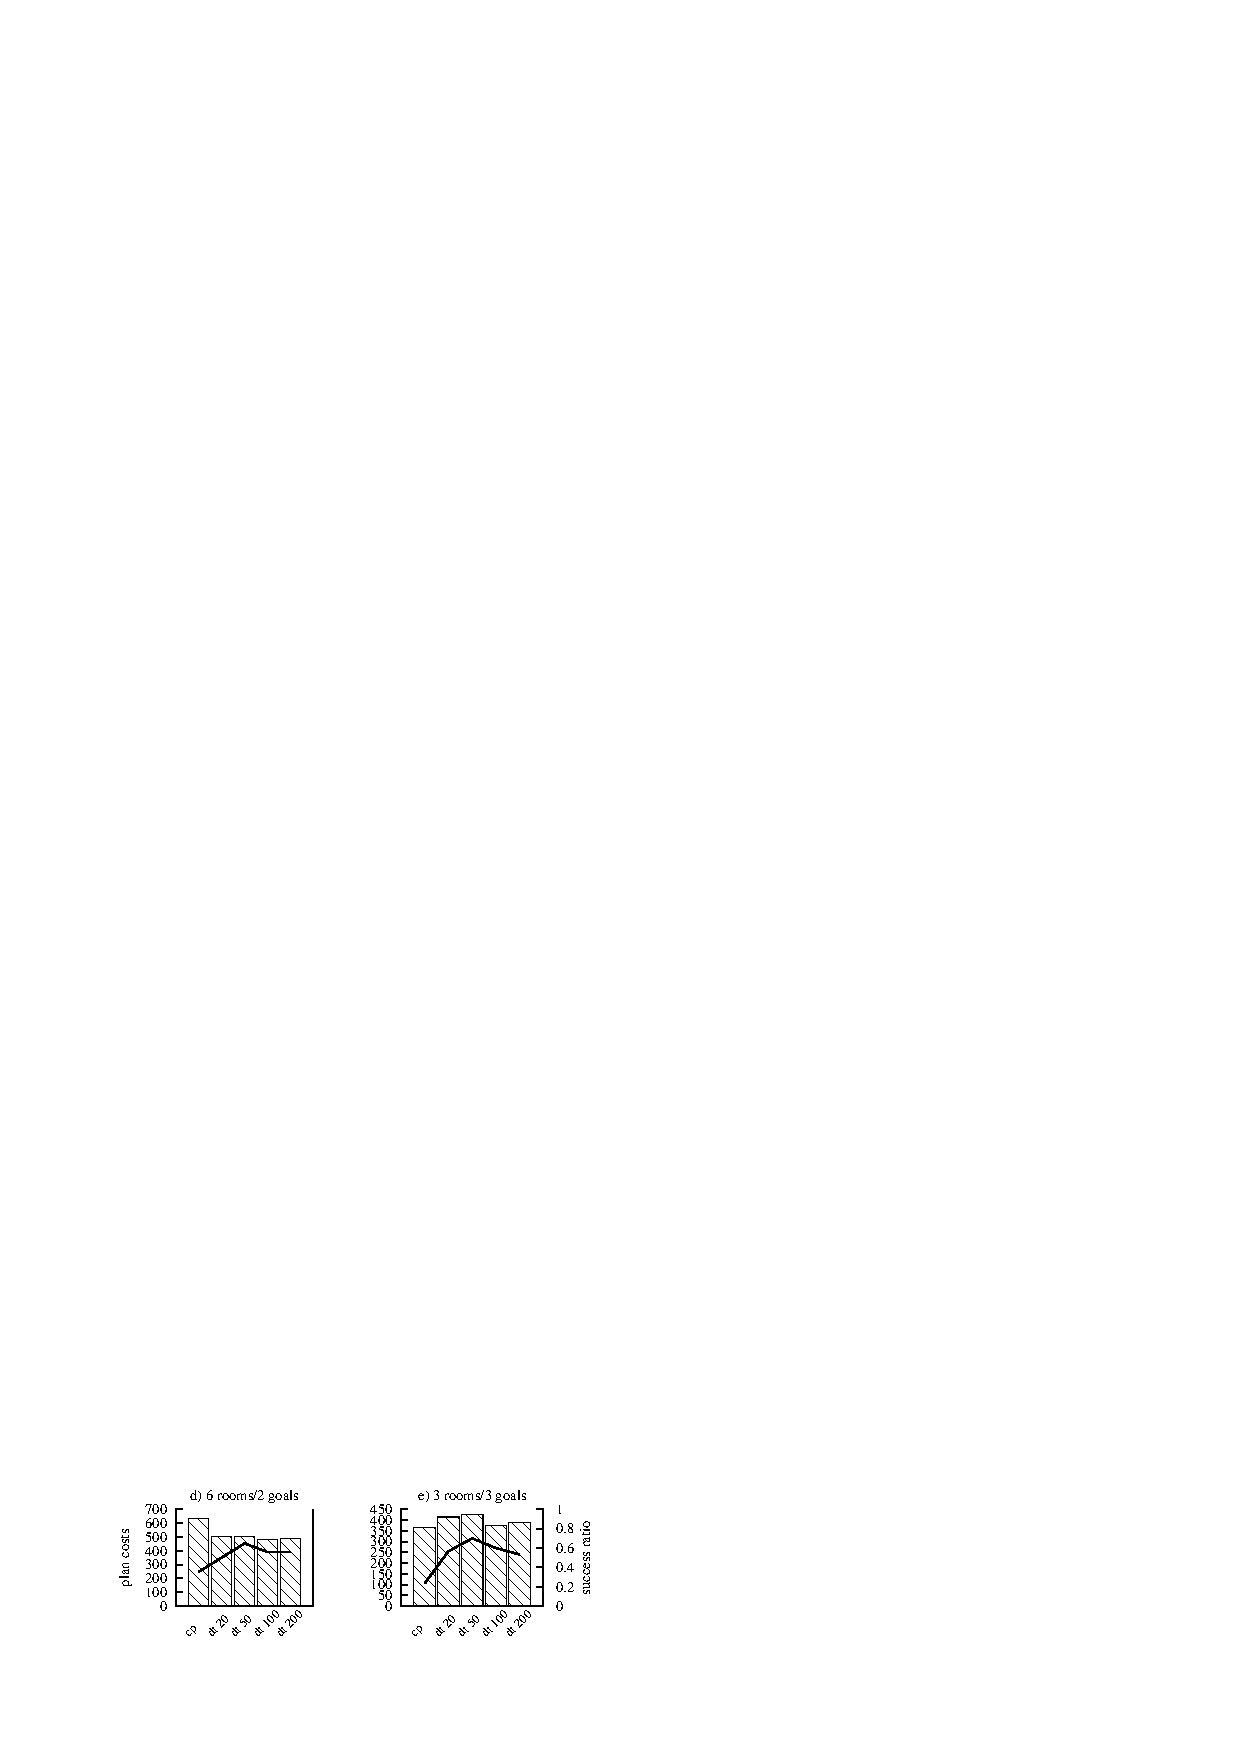
\includegraphics{dora56-quality}\hfill
  \vspace{2mm}
  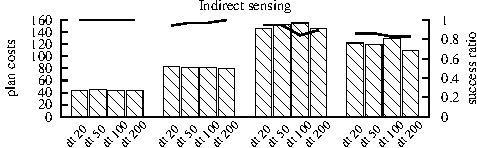
\includegraphics{dora-cat-quality}\hfill
  \caption{Average plan costs and number of successful runs.}
  \label{fig:results-quality}
\end{figure}


%% Figure \ref{fig:results-quality} shows the average costs of the
%% executed plans as well as the percentage of solvable tasks that were
%% actually solved by the planner. 


Our experimental results are summarised in
Figure~\ref{fig:results-time} and Figure~\ref{fig:results-quality}. We
find that the time spent on contingent planning increases steeply as
the abstraction $\bstate_0$ becomes more refined. For coarse initial
configurations, the cost of contingent planning is compensated by the
decrease of time spent in Fast Downward. Addressing success ratios and
plan costs, for objects that can be easily detected there is little
gain in using a decision-theoretic planner, as the greedy sensing
approach by the baseline is sufficient. With decreasing sensor
reliability contingent planning pays off.%% : while the resulting plans are still
%% longer on average, the impact on the number of solved tasks was much
%% smaller than for the baseline system.  Less aggressive abstraction
of the initial configuration results in longer runtimes. In our
scenario it is worthwhile being assumptively aggressive.  We suppose
the relatively high success rate irrespective of the coarseness of the
initial configuration indicates the effectiveness of using conditional
entropy to guide abstraction refinement.

We find that abstraction has little impact on plan
costs and success rate in our scenario. Increasing the size of the
initial abstract belief beyond 50 states rarely pays off, because
while additional information may facilitate better plans, the indirect
sensing tests report the same result. Here, we only really see an
impact in terms of the runtime of contingent planning. 

% We believe that a part of the improvement is due to the segmentation of
% the plan into several subtask, essentially performing hierarchical
% planning. Especially when the continual planner performs badly this is
% a huge gain.

%%% Local Variables: 
%%% mode: latex
%%% TeX-master: "moritz_2011"
%%% End: 
